\documentclass{standalone}
\usepackage{tikz}
\usetikzlibrary{patterns, positioning}
\usepackage[sfdefault]{ClearSans} %% option 'sfdefault' activates Clear Sans as the default text font
\usepackage[T1]{fontenc}

\begin{document}
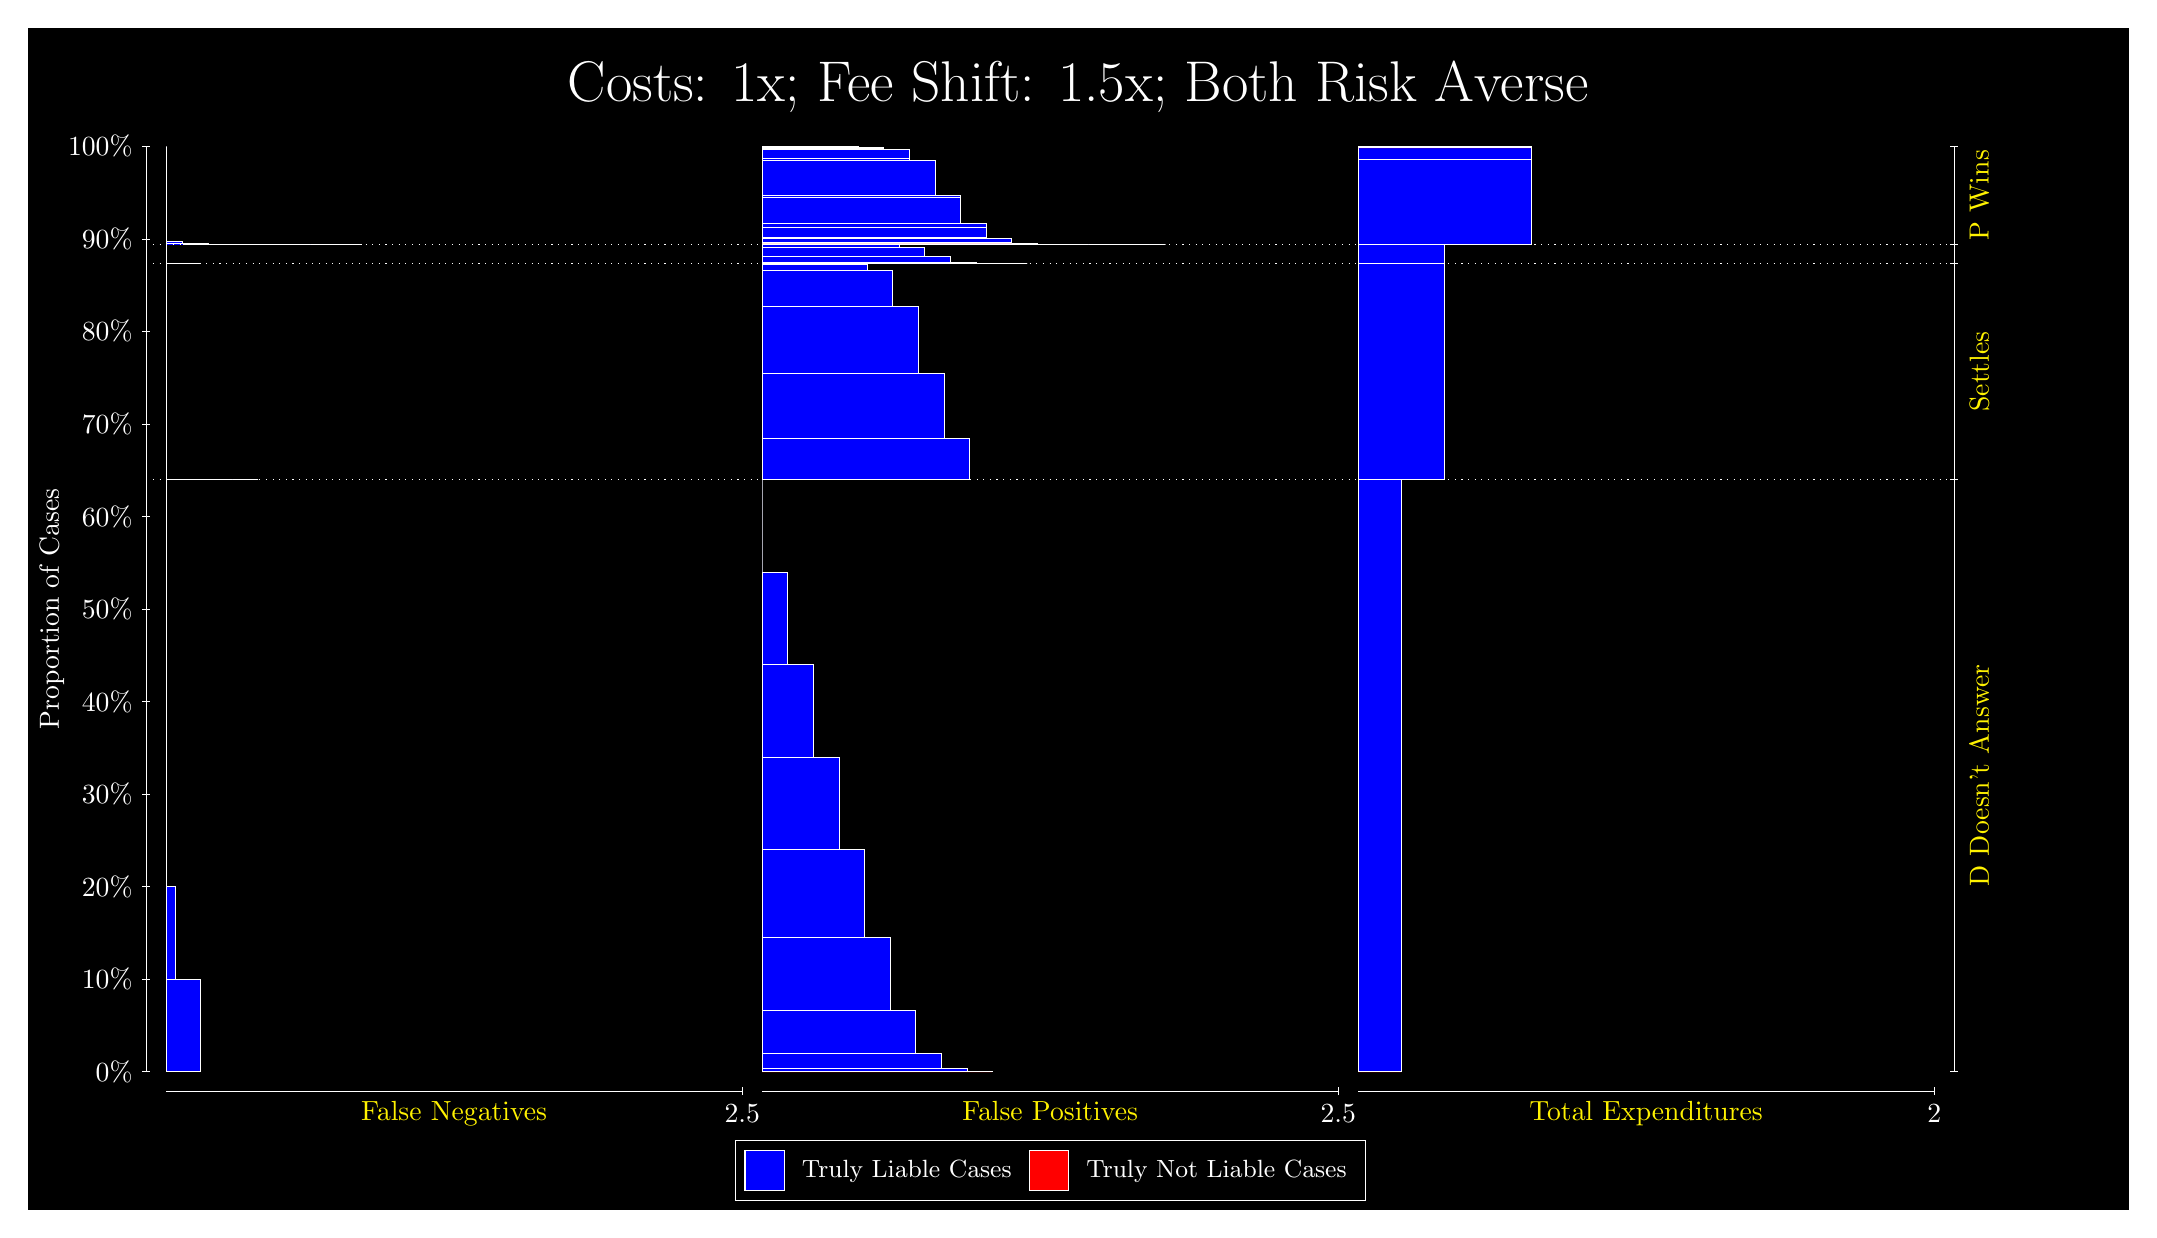
\begin{tikzpicture}
\draw[fill=black] (0,0) rectangle (26.667,15);
\draw[text=white] (0,13.5) rectangle (26.667,15) node[midway] {\huge Costs: 1x; Fee Shift: 1.5x; Both Risk Averse};
\draw[white, very thin] (1.5,1.75) -- (1.5,13.5);
\node[rotate=90, text=white, anchor=center] at (0.3, 7.625) {Proportion of Cases};
\draw[white, very thin] (1.45,1.75) -- (1.55,1.75);
\node[text=white, anchor=east] at (1.45, 1.75) {0\%};
\draw[white, very thin] (1.45,2.925) -- (1.55,2.925);
\node[text=white, anchor=east] at (1.45, 2.925) {10\%};
\draw[white, very thin] (1.45,4.1) -- (1.55,4.1);
\node[text=white, anchor=east] at (1.45, 4.1) {20\%};
\draw[white, very thin] (1.45,5.275) -- (1.55,5.275);
\node[text=white, anchor=east] at (1.45, 5.275) {30\%};
\draw[white, very thin] (1.45,6.45) -- (1.55,6.45);
\node[text=white, anchor=east] at (1.45, 6.45) {40\%};
\draw[white, very thin] (1.45,7.625) -- (1.55,7.625);
\node[text=white, anchor=east] at (1.45, 7.625) {50\%};
\draw[white, very thin] (1.45,8.8) -- (1.55,8.8);
\node[text=white, anchor=east] at (1.45, 8.8) {60\%};
\draw[white, very thin] (1.45,9.975) -- (1.55,9.975);
\node[text=white, anchor=east] at (1.45, 9.975) {70\%};
\draw[white, very thin] (1.45,11.15) -- (1.55,11.15);
\node[text=white, anchor=east] at (1.45, 11.15) {80\%};
\draw[white, very thin] (1.45,12.325) -- (1.55,12.325);
\node[text=white, anchor=east] at (1.45, 12.325) {90\%};
\draw[white, very thin] (1.45,13.5) -- (1.55,13.5);
\node[text=white, anchor=east] at (1.45, 13.5) {100\%};

\draw[white, very thin] (24.457,1.75) -- (24.457,13.5);
\draw[white, very thin] (24.407,1.75) -- (24.507,1.75);
\node[anchor=west] at (24.407, 1.75) {};
\draw[white, very thin] (24.407,9.2691) -- (24.507,9.2691);
\node[anchor=west] at (24.407, 9.2691) {};
\draw[white, very thin] (24.407,12.012) -- (24.507,12.012);
\node[anchor=west] at (24.407, 12.012) {};
\draw[white, very thin] (24.407,12.256) -- (24.507,12.256);
\node[anchor=west] at (24.407, 12.256) {};
\draw[white, very thin] (24.407,13.5) -- (24.507,13.5);
\node[anchor=west] at (24.407, 13.5) {};

\draw[white, very thin, fill=blue] (1.75,1.75) rectangle (2.1891,2.925);
\draw[white, very thin, fill=blue] (1.75,2.925) rectangle (1.8638,4.1);
\draw[white, very thin, fill=red] (1.75,4.1) rectangle (1.75,4.1);
\draw[white, very thin, fill=blue] (1.75,4.1) rectangle (1.75,9.2691);
\draw[white, very thin, fill=blue] (1.75,9.2691) rectangle (2.921,9.2691);
\draw[white, very thin, fill=blue] (1.75,9.2691) rectangle (2.5957,9.2691);
\draw[white, very thin, fill=blue] (1.75,9.2691) rectangle (2.2705,9.2691);
\draw[white, very thin, fill=blue] (1.75,9.2691) rectangle (1.9452,9.2692);
\draw[white, very thin, fill=red] (1.75,9.2692) rectangle (1.75,9.2692);
\draw[white, very thin, fill=blue] (1.75,9.2692) rectangle (1.75,12.012);
\draw[white, very thin, fill=blue] (1.75,12.012) rectangle (2.1891,12.012);
\draw[white, very thin, fill=blue] (1.75,12.012) rectangle (1.8638,12.012);
\draw[white, very thin, fill=red] (1.75,12.012) rectangle (1.75,12.012);
\draw[white, very thin, fill=blue] (1.75,12.012) rectangle (1.75,12.256);
\draw[white, very thin, fill=blue] (1.75,12.256) rectangle (4.2384,12.256);
\draw[white, very thin, fill=blue] (1.75,12.256) rectangle (3.9131,12.256);
\draw[white, very thin, fill=blue] (1.75,12.256) rectangle (3.5878,12.256);
\draw[white, very thin, fill=blue] (1.75,12.256) rectangle (3.2626,12.256);
\draw[white, very thin, fill=blue] (1.75,12.256) rectangle (3.2626,12.256);
\draw[white, very thin, fill=blue] (1.75,12.256) rectangle (2.9373,12.256);
\draw[white, very thin, fill=blue] (1.75,12.256) rectangle (2.9373,12.256);
\draw[white, very thin, fill=blue] (1.75,12.256) rectangle (2.9373,12.256);
\draw[white, very thin, fill=blue] (1.75,12.256) rectangle (2.612,12.256);
\draw[white, very thin, fill=blue] (1.75,12.256) rectangle (2.612,12.257);
\draw[white, very thin, fill=blue] (1.75,12.257) rectangle (2.2867,12.257);
\draw[white, very thin, fill=blue] (1.75,12.257) rectangle (2.2867,12.257);
\draw[white, very thin, fill=blue] (1.75,12.257) rectangle (2.2867,12.263);
\draw[white, very thin, fill=blue] (1.75,12.263) rectangle (1.9614,12.264);
\draw[white, very thin, fill=blue] (1.75,12.264) rectangle (1.9614,12.295);
\draw[white, very thin, fill=blue] (1.75,12.295) rectangle (1.9614,12.295);
\draw[white, very thin, fill=red] (1.75,12.295) rectangle (1.75,12.295);
\draw[white, very thin, fill=blue] (1.75,12.295) rectangle (1.75,13.5);
\draw[white, very thin, fill=red] (9.3189,1.75) rectangle (12.246,1.75);
\draw[white, very thin, fill=blue] (9.3189,1.75) rectangle (12.246,1.7544);
\draw[white, very thin, fill=blue] (9.3189,1.7544) rectangle (11.921,1.7924);
\draw[white, very thin, fill=blue] (9.3189,1.7924) rectangle (11.596,1.9842);
\draw[white, very thin, fill=blue] (9.3189,1.9842) rectangle (11.271,2.5245);
\draw[white, very thin, fill=blue] (9.3189,2.5245) rectangle (10.945,3.4492);
\draw[white, very thin, fill=blue] (9.3189,3.4492) rectangle (10.62,4.5738);
\draw[white, very thin, fill=blue] (9.3189,4.5738) rectangle (10.295,5.7443);
\draw[white, very thin, fill=blue] (9.3189,5.7443) rectangle (9.9694,6.9191);
\draw[white, very thin, fill=blue] (9.3189,6.9191) rectangle (9.6442,8.0941);
\draw[white, very thin, fill=blue] (9.3189,8.0941) rectangle (9.3189,9.2691);
\draw[white, very thin, fill=red] (9.3189,9.2691) rectangle (11.954,9.2691);
\draw[white, very thin, fill=blue] (9.3189,9.2691) rectangle (11.954,9.7888);
\draw[white, very thin, fill=blue] (9.3189,9.7888) rectangle (11.628,10.617);
\draw[white, very thin, fill=blue] (9.3189,10.617) rectangle (11.303,11.472);
\draw[white, very thin, fill=blue] (9.3189,11.472) rectangle (10.978,11.921);
\draw[white, very thin, fill=blue] (9.3189,11.921) rectangle (10.653,12.007);
\draw[white, very thin, fill=blue] (9.3189,12.007) rectangle (10.327,12.012);
\draw[white, very thin, fill=blue] (9.3189,12.012) rectangle (10.002,12.012);
\draw[white, very thin, fill=blue] (9.3189,12.012) rectangle (9.6767,12.012);
\draw[white, very thin, fill=blue] (9.3189,12.012) rectangle (9.3514,12.012);
\draw[white, very thin, fill=blue] (9.3189,12.012) rectangle (9.3189,12.012);
\draw[white, very thin, fill=red] (9.3189,12.012) rectangle (12.686,12.012);
\draw[white, very thin, fill=blue] (9.3189,12.012) rectangle (12.686,12.012);
\draw[white, very thin, fill=blue] (9.3189,12.012) rectangle (12.36,12.012);
\draw[white, very thin, fill=blue] (9.3189,12.012) rectangle (12.035,12.022);
\draw[white, very thin, fill=blue] (9.3189,12.022) rectangle (11.71,12.1);
\draw[white, very thin, fill=blue] (9.3189,12.1) rectangle (11.384,12.213);
\draw[white, very thin, fill=blue] (9.3189,12.213) rectangle (11.059,12.252);
\draw[white, very thin, fill=blue] (9.3189,12.252) rectangle (10.734,12.256);
\draw[white, very thin, fill=blue] (9.3189,12.256) rectangle (10.409,12.256);
\draw[white, very thin, fill=blue] (9.3189,12.256) rectangle (10.083,12.256);
\draw[white, very thin, fill=blue] (9.3189,12.256) rectangle (9.758,12.256);
\draw[white, very thin, fill=red] (9.3189,12.256) rectangle (14.442,12.256);
\draw[white, very thin, fill=blue] (9.3189,12.256) rectangle (14.442,12.256);
\draw[white, very thin, fill=red] (9.3189,12.256) rectangle (14.117,12.256);
\draw[white, very thin, fill=blue] (9.3189,12.256) rectangle (14.117,12.256);
\draw[white, very thin, fill=red] (9.3189,12.256) rectangle (13.792,12.256);
\draw[white, very thin, fill=blue] (9.3189,12.256) rectangle (13.792,12.256);
\draw[white, very thin, fill=blue] (9.3189,12.256) rectangle (13.466,12.256);
\draw[white, very thin, fill=red] (9.3189,12.256) rectangle (13.466,12.256);
\draw[white, very thin, fill=blue] (9.3189,12.256) rectangle (13.466,12.256);
\draw[white, very thin, fill=red] (9.3189,12.256) rectangle (13.141,12.256);
\draw[white, very thin, fill=blue] (9.3189,12.256) rectangle (13.141,12.258);
\draw[white, very thin, fill=blue] (9.3189,12.258) rectangle (13.141,12.259);
\draw[white, very thin, fill=red] (9.3189,12.259) rectangle (12.816,12.259);
\draw[white, very thin, fill=blue] (9.3189,12.259) rectangle (12.816,12.272);
\draw[white, very thin, fill=blue] (9.3189,12.272) rectangle (12.816,12.273);
\draw[white, very thin, fill=blue] (9.3189,12.273) rectangle (12.49,12.278);
\draw[white, very thin, fill=red] (9.3189,12.278) rectangle (12.49,12.278);
\draw[white, very thin, fill=blue] (9.3189,12.278) rectangle (12.49,12.337);
\draw[white, very thin, fill=blue] (9.3189,12.337) rectangle (12.165,12.349);
\draw[white, very thin, fill=red] (9.3189,12.349) rectangle (12.165,12.349);
\draw[white, very thin, fill=blue] (9.3189,12.349) rectangle (12.165,12.477);
\draw[white, very thin, fill=blue] (9.3189,12.477) rectangle (12.165,12.524);
\draw[white, very thin, fill=red] (9.3189,12.524) rectangle (11.84,12.524);
\draw[white, very thin, fill=blue] (9.3189,12.524) rectangle (11.84,12.853);
\draw[white, very thin, fill=blue] (9.3189,12.853) rectangle (11.84,12.879);
\draw[white, very thin, fill=blue] (9.3189,12.879) rectangle (11.84,12.881);
\draw[white, very thin, fill=red] (9.3189,12.881) rectangle (11.515,12.881);
\draw[white, very thin, fill=blue] (9.3189,12.881) rectangle (11.515,13.322);
\draw[white, very thin, fill=blue] (9.3189,13.322) rectangle (11.515,13.322);
\draw[white, very thin, fill=blue] (9.3189,13.322) rectangle (11.189,13.348);
\draw[white, very thin, fill=blue] (9.3189,13.348) rectangle (11.189,13.461);
\draw[white, very thin, fill=blue] (9.3189,13.461) rectangle (11.189,13.461);
\draw[white, very thin, fill=blue] (9.3189,13.461) rectangle (10.864,13.473);
\draw[white, very thin, fill=blue] (9.3189,13.473) rectangle (10.864,13.492);
\draw[white, very thin, fill=blue] (9.3189,13.492) rectangle (10.864,13.493);
\draw[white, very thin, fill=blue] (9.3189,13.493) rectangle (10.539,13.495);
\draw[white, very thin, fill=blue] (9.3189,13.495) rectangle (10.539,13.499);
\draw[white, very thin, fill=blue] (9.3189,13.499) rectangle (10.539,13.499);
\draw[white, very thin, fill=blue] (9.3189,13.499) rectangle (10.539,13.499);
\draw[white, very thin, fill=blue] (9.3189,13.499) rectangle (10.213,13.5);
\draw[white, very thin, fill=blue] (9.3189,13.5) rectangle (10.213,13.5);
\draw[white, very thin, fill=blue] (9.3189,13.5) rectangle (9.8881,13.5);
\draw[white, very thin, fill=blue] (9.3189,13.5) rectangle (9.8881,13.5);
\draw[white, very thin, fill=blue] (9.3189,13.5) rectangle (9.5628,13.5);
\draw[white, very thin, fill=blue] (9.3189,13.5) rectangle (9.5628,13.5);
\draw[white, very thin, fill=blue] (9.3189,13.5) rectangle (9.3189,13.5);
\draw[white, very thin, fill=red] (16.888,1.75) rectangle (17.437,1.75);
\draw[white, very thin, fill=blue] (16.888,1.75) rectangle (17.437,9.2691);
\draw[white, very thin, fill=red] (16.888,9.2691) rectangle (17.986,9.2691);
\draw[white, very thin, fill=blue] (16.888,9.2691) rectangle (17.986,12.012);
\draw[white, very thin, fill=red] (16.888,12.012) rectangle (17.986,12.012);
\draw[white, very thin, fill=blue] (16.888,12.012) rectangle (17.986,12.256);
\draw[white, very thin, fill=red] (16.888,12.256) rectangle (19.083,12.256);
\draw[white, very thin, fill=blue] (16.888,12.256) rectangle (19.083,13.337);
\draw[white, very thin, fill=red] (16.888,13.337) rectangle (19.083,13.337);
\draw[white, very thin, fill=blue] (16.888,13.337) rectangle (19.083,13.483);
\draw[white, very thin, fill=red] (16.888,13.483) rectangle (19.083,13.483);
\draw[white, very thin, fill=blue] (16.888,13.483) rectangle (19.083,13.5);
\draw[white, dotted] (1.5,9.2691) -- (24.457,9.2691);
\draw[white, dotted] (1.5,12.012) -- (24.457,12.012);
\draw[white, dotted] (1.5,12.256) -- (24.457,12.256);
\draw[white, very thin] (1.75,1.5) -- (9.0689,1.5);
\node[text=yellow, anchor=north] at (5.4094, 1.5) {False Negatives};
\draw[white, very thin] (9.0689,1.45) -- (9.0689,1.55);
\node[text=white, anchor=north] at (9.0689, 1.45) {2.5};

\draw[white, very thin] (9.3189,1.5) -- (16.638,1.5);
\node[text=yellow, anchor=north] at (12.978, 1.5) {False Positives};
\draw[white, very thin] (16.638,1.45) -- (16.638,1.55);
\node[text=white, anchor=north] at (16.638, 1.45) {2.5};

\draw[white, very thin] (16.888,1.5) -- (24.207,1.5);
\node[text=yellow, anchor=north] at (20.547, 1.5) {Total Expenditures};
\draw[white, very thin] (24.207,1.45) -- (24.207,1.55);
\node[text=white, anchor=north] at (24.207, 1.45) {2};

\node[text=yellow, centered, rotate=90] at (24.777, 5.5096) {D Doesn't Answer};
\node[text=yellow, centered, rotate=90] at (24.777, 10.64) {Settles};

\node[text=yellow, centered, rotate=90] at (24.777, 12.878) {P Wins};

\draw (12.978300999999998,1.5) node[draw=none] (baseCoordinate) {};
\begin{scope}[align=center]
        \matrix[scale=0.5, draw=white, below=0.5cm of baseCoordinate, nodes={draw}, column sep=0.1cm]{
            \node[rectangle, draw, minimum width=0.5cm, minimum height=0.5cm, fill=blue] {}; &
            \node[draw=none, font=\small, text=white] (B) {Truly Liable Cases}; &
            \node[rectangle, draw, minimum width=0.5cm, minimum height=0.5cm, fill=red] {}; &
            \node[draw=none, font=\small, text=white] (B) {Truly Not Liable Cases}; \\
            };
\end{scope}

\end{tikzpicture}
\end{document}